\subsection{Web Audio Demo Application} \label{section:methodJavascript}

To develop the extension for the e-learning platform Easydrum, the developed algorithm has to run in web browsers with JavaScript. To realize that, the Web Midi API and the WebRTC shall be used. In the following, a sample application is described, which receives an audio stream from a microphone and draws each received audio frame onto a canvas element. A screenshot of the application is shown in figure \ref{fig:exampleAppScreenshot}.

\begin{figure}[ht]
	\centering
	\subfloat[Screenshot.]{
		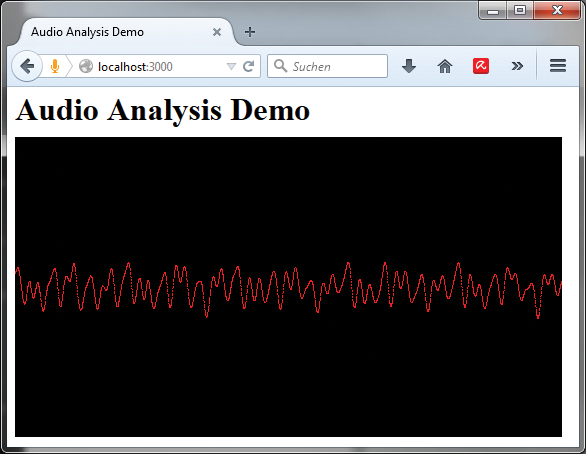
\includegraphics[width=7.2cm]{images/exampleappscreen.png}
		\label{fig:exampleAppScreenshot}
	}
	\qquad
	\subfloat[Basic architecture.]{
		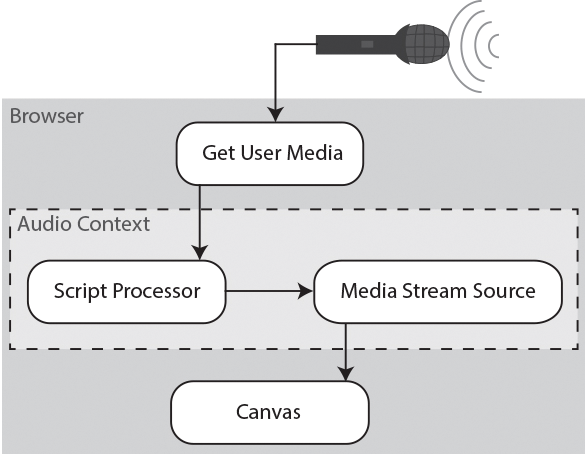
\includegraphics[width=7.2cm]{images/exampleapparchitecture.png}
		\label{fig:exampleAppArchitecture}
	}
	\caption{
		Sample web application.
	}
	\label{fig:exampleApp}
\end{figure}

As displayed in figure \ref{fig:exampleAppArchitecture}, the application is built of two web audio API nodes, a canvas element and a function that receives the microphone input via the WebRTC. The two nodes that are connected to each other, are a media stream source node and a custom script processor node. The media stream source node receives the media stream from a microphone through the WebRTCs function \lstinline{navigator.getUserMedia}. It passes on the data to the script processor, which saves the audio wave data. Finally, the audio wave data is used by the canvas to draw the visualization. 

\begin{sloppypar}
The application is built of two files. These are a basic HTML file and a JavaScript file, which is loaded into the HTML file. The JavaScript file is built of six functions. After the document is loaded, three initial functions are called. They initialize the visualization, the audio context and nodes and the microphone input. The three functions are called \lstinline{initVisualization}, \lstinline{initAudioContext} and \lstinline{initMicrophoneInput}. Finally, the visualization is started. Next to the initial functions, there are three other functions used as callbacks for handling the microphone input, processing the incoming audio stream and updating the visualization on the canvas. These functions are \lstinline{handleMicrophoneInput}, \lstinline{onAudioProcess} and \lstinline{updateVisualization}. The function \lstinline{initVisualization}, which is shown in listing \ref{lst:demo1}, appends a canvas element into the body of the HTML page. It gives the element the width of the browser window minus 25px and a height of 300px and the background color black. It saves the canvas element itself and it's 2d-context as variables \lstinline{c} and \lstinline{ctx}. Furthermore, \lstinline{initVisualization} prepares the function \lstinline{window.requestAnimationFrame} to run with the same function call in different browsers. This is required because there are browsers which use the function \lstinline{window.webkitRequestAnimationFrame} instead of \lstinline{window.requestAnimationFrame}. The function is needed to update the visualization and adapt the frame rate to the calculation power of the processor. 
\end{sloppypar}

\begin{lstlisting}[caption={Web Audio Demo: Initialize visualization.},label={lst:demo1}, language=JavaScript]
function initVisualization() {
		if (!window.requestAnimationFrame)
			window.requestAnimationFrame = window.webkitRequestAnimationFrame;

		\$("body").append('<canvas id="visualisation" width="'+(window.innerWidth-25)+'" height="300" style="background:black;"></canvas><br>');
		c = document.getElementById("visualisation");
		ctx = c.getContext("2d");
}
\end{lstlisting}

By the function \lstinline{initAudioContext}, the audio context and the script processor node are created and saved in global variables. The script processor node receives three arguments. The first one is the buffer size, which defines the size of the frames in the audio stream. The second one is the number of input channels and the third one the number of output channels. In the example, the buffer size is set to a size of 4096 by a globally defined variable \lstinline{BUFFER\_SIZE}. The number of channels for input and output are set to one. After the script processor node is created, the function \lstinline{onAudioProcess} is set as callback for the script processor's function \lstinline{onaudioprocess}. Thus, the function is applied to every buffered data instance in the data stream. The JavaScript code for \lstinline{initAudioContext} and \lstinline{onAudioProcess} is displayed in listing \ref{lst:demo2}.

\begin{lstlisting}[caption={Web Audio Demo: Initialize audio context.},label={lst:demo2}, language=JavaScript]
function initAudioContext() {
    audioCtx = new AudioContext();   
    scriptProcessorNode = audioCtx.createScriptProcessor(BUFFER_SIZE, 1, 1); 
    scriptProcessorNode.onaudioprocess = onAudioProcess;
}
function onAudioProcess(e){
    data = new Float32Array(BUFFER_SIZE);
    data = e.inputBuffer.getChannelData (0);
}
\end{lstlisting}

The third initial function, \lstinline{initMicrophoneInput}, connects the browser to a microphone by the use of the WebRTCs function \lstinline{navigator.getUserMedia}. Before the function is used, its function name is configured to work with different browsers in the same manner as it was done for \lstinline{window.requestAnimationFrame}. If it is not supported in the used browser, there is an error message printed to the JavaScript console. The function \lstinline{navigator.getUserMedia} receives three arguments. The first argument contains options as DOM String. The second argument contains a callback that is executed if the audio stream is received successfully. The last argument is optional and contains another callback function that is executed if an error occurs while trying to connect to the microphone. In the sample application, the options include \lstinline{audio:true} and \lstinline{video:false}, which means that only audio stream data will be received. The function \lstinline{handleMicrophoneInput} is transferred as success call-back. If an error occurs while connecting, a message is printed to the console. The function \lstinline{handleMicrophoneInput} receives the audio stream by the navigator. It creates the media stream source node, which is saved in the global variable \lstinline{microphoneNode}. The media stream is transferred to this media stream source node as argument. It is connected to the script processor node, which processes each data instance of the media stream. The source code for \lstinline{initMicrophoneInput} and \lstinline{handleMicrophoneInput} is shown in listing \ref{lst:demo3}.

\begin{lstlisting}[caption={Web Audio Demo: Initialize microphone input.},label={lst:demo3}, language=JavaScript]
function initMicrophoneInput(){
    if (!!(navigator.getUserMedia || navigator.webkitGetUserMedia || navigator.mozGetUserMedia || navigator.msGetUserMedia)) {      
        navigator.getUserMedia = navigator.getUserMedia || navigator.webkitGetUserMedia || navigator.mozGetUserMedia || navigator.msGetUserMedia;
    } else {
        alert('getUserMedia() is not supported in your browser');        
    }
    navigator.getUserMedia({audio: true, video: false}, 
        handleMicrophoneInput, 
        function () {
            console.log('capturing microphone data failed!');
            console.log(evt);
        }
    );
}
function handleMicrophoneInput(stream){
    console.log("capturing microphone data ...");
    microphoneNode = audioCtx.createMediaStreamSource(stream);
    microphoneNode.connect(scriptProcessorNode);   
}
\end{lstlisting}

After all components are initialized, the visualization on the canvas element is started by calling \lstinline{rafID = window.requestAnimationFrame(updateVisualization)}. Thereby, the function \lstinline{updateVisualization} is passed as callback function. Thus, it is processed for every loaded frame. The function gets the last processed audio frame saved by the script processor node and draws the containing wave on the canvas. Thereby, each data point in the audio frame array is drawn as rectangle with a height and a width of one pixel. 

\begin{lstlisting}[caption={Web Audio Demo: Update visualization.},label={lst:demo4}, language=JavaScript]
function updateVisualization() {
    var width = c.width;
    var height = c.height;
    var scale_x = BUFFER_SIZE/width;
    var _data = data; // contains sine wave with values beween -1 and 1
    ctx.clearRect(0, 0, c.width, c.height);
    for (var i = 0; i < BUFFER_SIZE; i++) {
        var value = _data[i]*height/2;
        var left = Math.round(i/scale_x);
        var top = 0;
        if(value < 0){
            value = Math.abs(value);
            top = Math.round(value + height/2);
        }else{
            top = Math.round(height/2 - value);
        }
        ctx.fillStyle = "red";
        ctx.fillRect(left, top, 1, 1);
    }
    //update visualisation
    rafID = window.requestAnimationFrame(updateVisualization);
}
\end{lstlisting}


To view the sample application, it has to run on a server because otherwise the function \lstinline{navigator.getUserMedia} of the WebRTC doesn’t work. The application is tested with Mozilla Firefox version 37.0.2 on Windows 7.
